\indent Para verificar el correcto funcionamiento de nuestro algoritmo , elaboramos disversos tests,
los cuales ser\'an enunciados a continuaci\'on.\\

\begin{center}
 \textbf{No existe camino para atravezar el laberinto}
\end{center}

Este caso se da cuando en cualquier camino nos encontramos con paredes irrompibles sin la posibilidad de esquivarlas\\

 Con un:
 
\vspace*{0.3cm} \vspace*{0.3cm}
  \begin{center}
 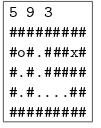
\includegraphics[scale=0.65]{./EJ1/ej1sinsolucion.jpeg}
\\{$Ejemplo$ \ 1.1.1 - $Caso$ $Sin$ $Soluci$\'on}
  \end{center}
  \vspace*{0.3cm}

El grafo que representa a este tipo es de la siguiente forma:\\

\vspace*{0.3cm} \vspace*{0.3cm}
  \begin{center}
 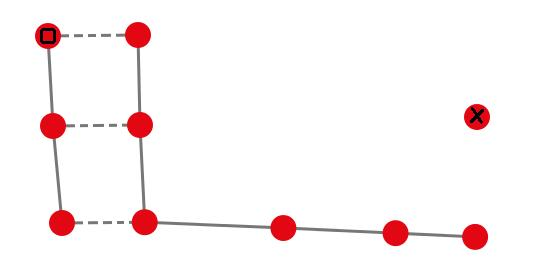
\includegraphics[scale=0.5]{./EJ1/ej1grafosinsolucion.jpeg}
 \\{$Ejemplo$ \ 1.1.2 - $Caso$ $Sin$ $Soluci$\'on}
  \end{center}
  \vspace*{0.3cm}


 \begin{center}
 \textbf{Existe un camino sin atravesar paredes para recorrer todo el laberinto}
\end{center}

Esta versi\'on se da cuando $P' = P$ con $P' = P - atravezadas$. 

 Con un:
 
\vspace*{0.3cm} \vspace*{0.3cm}
  \begin{center}
 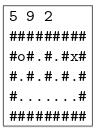
\includegraphics[scale=0.65]{./EJ1/ej1solucionsinpared.jpeg}
 \\{$Ejemplo$ \ 1.2.1 - $Caso$ $Sin$ $Romper$ $Paredes$}
  \end{center}
  \vspace*{0.3cm}

El grafo que representa a este tipo es de la siguiente forma:\\

\vspace*{0.3cm} \vspace*{0.3cm}
  \begin{center}
 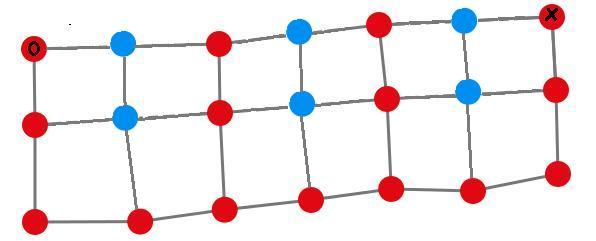
\includegraphics[scale=0.5]{./EJ1/ej1grafosolucionsinpared.jpeg}
 \\{$Ejemplo$ \ 1.2.2 - $Caso$ $Sin$ $Romper$ $Paredes$}
  \end{center}
  \vspace*{0.3cm}

  
\begin{center}
 \textbf{Rompiendo todas las paredes posibles para pasar el laberinto}
\end{center}

Este caso se da cuando $P' = 0$ con $P' = P - atravezadas$ 

 Con un:
 
\vspace*{0.3cm} \vspace*{0.3cm}
  \begin{center}
 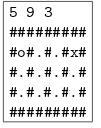
\includegraphics[scale=0.65]{./EJ1/ej1rompertodasparedes.jpeg}
\\ {$Ejemplo$ \ 1.3.1 - $Caso$ $Rompiendo$ $Todas$ $Paredes$ $Las$ $Posibles$}
  \end{center}
  \vspace*{0.3cm}

El grafo que representa a este tipo es de la siguiente forma:\\

\vspace*{0.3cm} \vspace*{0.3cm}
  \begin{center}
 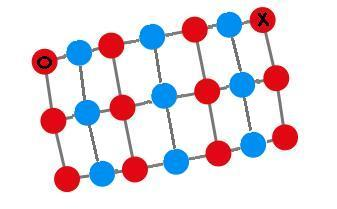
\includegraphics[scale=0.5]{./EJ1/ej1grafosolucionconpared.jpeg}
 \\{$Ejemplo$ \ 1.3.2 - $Caso$ $Rompiendo$ $Todas$ $Paredes$ $Las$ $Posibles$}
  \end{center}
  \vspace*{0.3cm}


\begin{center}
 \textbf{Rompiendo una cantidad menor de paredes posibles para pasar el laberinto}
\end{center}

Este caso se da cuando $P \geq P' \geq 0$ con $P' = P - atravezadas$, tambi\'en denominado caso random debido al desarrollo de nuestro algoritmo.\\


 Con un:
 
\vspace*{0.3cm} \vspace*{0.3cm}
  \begin{center}
 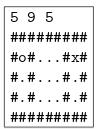
\includegraphics[scale=0.65]{./EJ1/ej1random.jpeg}
\\ {$Ejemplo$ \ 1.4.1 - $Caso$ $Random$}
  \end{center}
  \vspace*{0.3cm}

El grafo que representa a este tipo es de la siguiente forma:\\

\vspace*{0.3cm} \vspace*{0.3cm}
  \begin{center}
 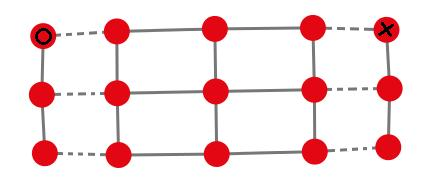
\includegraphics[scale=0.5]{./EJ1/ej1graforandom.jpeg}
 \\{$Ejemplo$ \ 1.4.2 - $Caso$ $Random$}
  \end{center}
  \vspace*{0.3cm}



\textbf{Aclaraciones:} 
\begin{itemize}
\item Nodo color celeste es una pared.
\end{itemize}
